%!TEX root = ../../main.tex


\begin{figure}[!htb]
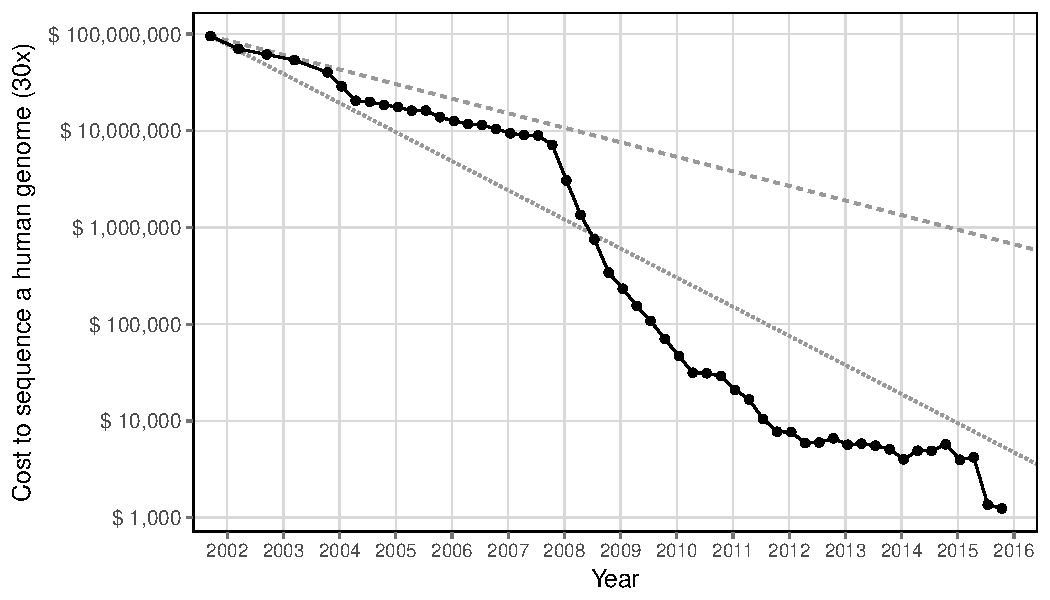
\includegraphics[width=\textwidth]{./img/ch1/cost_per_genome}
\Caption{Timeline of cost reduction in DNA sequencing}
{Technological improvements in whole-genome sequencing have led to drastic reductions in cost while simultaneously improving accuracy and speed of data generation.
The plot shows the development of price per human-sized genome sequenced at 30x depth (price given in US dollars) since the publication of the first draft sequence of the human genome in 2001.
The costs shown between 2001 and 2007 are based on the Sanger sequencing method (\emph{first-generation} methods); since 2008, costs are based on \emph{next-generation} technologies.
The hypothetically expected rate of cost reduction per genome is indicated according to Moore's law \citep{moore1965}; the price halves every \n{2} years (\emph{dashed}) or every year (\emph{dotted}).
Data provided by the \glsentryfull{nhgri}: \url{https://www.genome.gov/sequencingcostsdata/} \accessed{2017}{03}{15}.}
{fig:cost_per_genome}
\end{figure}
